\section{Interpretation}

The first angular analysis of \BdToKstmm has been interpreted both in context of placing constraints of the values of
the Wilson coefficients \C7, \C9 and \C10 ~\cite{Bobeth:2011nj}.
The constraints placed by measurements of electroweak penguin decays on the absolute 
magnitude of \C9 and \C10 are shown in Fig~\ref{fig:c9vsc10}.
\begin{figure}[tb]
\centering
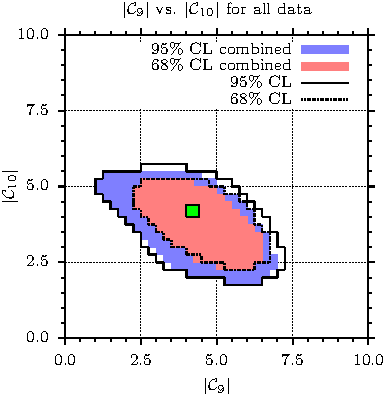
\includegraphics[width=0.48\columnwidth]{chapter5/figs/theo/fig-constraints-c9-c10-all-all-all-contour.pdf}
\caption{ Constraints on the $|\C9 |$ v.s. $|\C10 |$ using the measurements of electroweak penguin decays
 available towards the end of 2011. Taken from Ref.~\cite{Bobeth:2011nj}.~\label{fig:c9vsc10} }
\end{figure}
A second interpretation of \BdToKstmm in the context of similar heavy flavour decays has also placed constraints on 
the values of the Wilson coefficients using the results from the first and second angular analyses respectively
~\cite{Altmannshofer:2011gn,Altmannshofer:2012az}.
It is possible to see that the measurements presented in this chapter provide some of the most stringent constraints on
 the values of the Wilson coefficients from \bquark\to\squark decays.

